\documentclass[11pt]{article}

\usepackage[margin=1in]{geometry}
\usepackage{amsmath, amssymb}
\usepackage{graphicx}
\usepackage{subcaption}
\usepackage{listings}
\usepackage{xcolor}
\usepackage{hyperref}
\usepackage{booktabs}
\usepackage{placeins}
\usepackage{adjustbox}

\hypersetup{
  colorlinks=true,
  linkcolor=black,
  filecolor=magenta,
  urlcolor=blue,
  citecolor=black
}

\usepackage[capitalise,noabbrev]{cleveref}

\lstset{
    basicstyle=\ttfamily\small,
    breaklines=true,
    frame=single,
    numbers=left,
    numberstyle=\tiny,
    keywordstyle=\color{blue},
    commentstyle=\color{gray},
    tabsize=4
}

\title{\textbf{High Performance Parallel Computing \\ Homework 2}}
\author{Liam Pohlmann, Alex Shaffer}
\date{\today}

\begin{document}

\maketitle

\section{Problem 1}

% ---------------------------------------------------------------- verification
\subsection{Verification}


As demonstrated with \cref{fig:solution-contours,fig:max-error-versus-grid-size}, the implemeted algorithm converges to the correct solution with the expected quadratic convergence rate.

\begin{figure}[htbp]
  \centering
  \begin{subfigure}{0.49\textwidth}
    \centering
    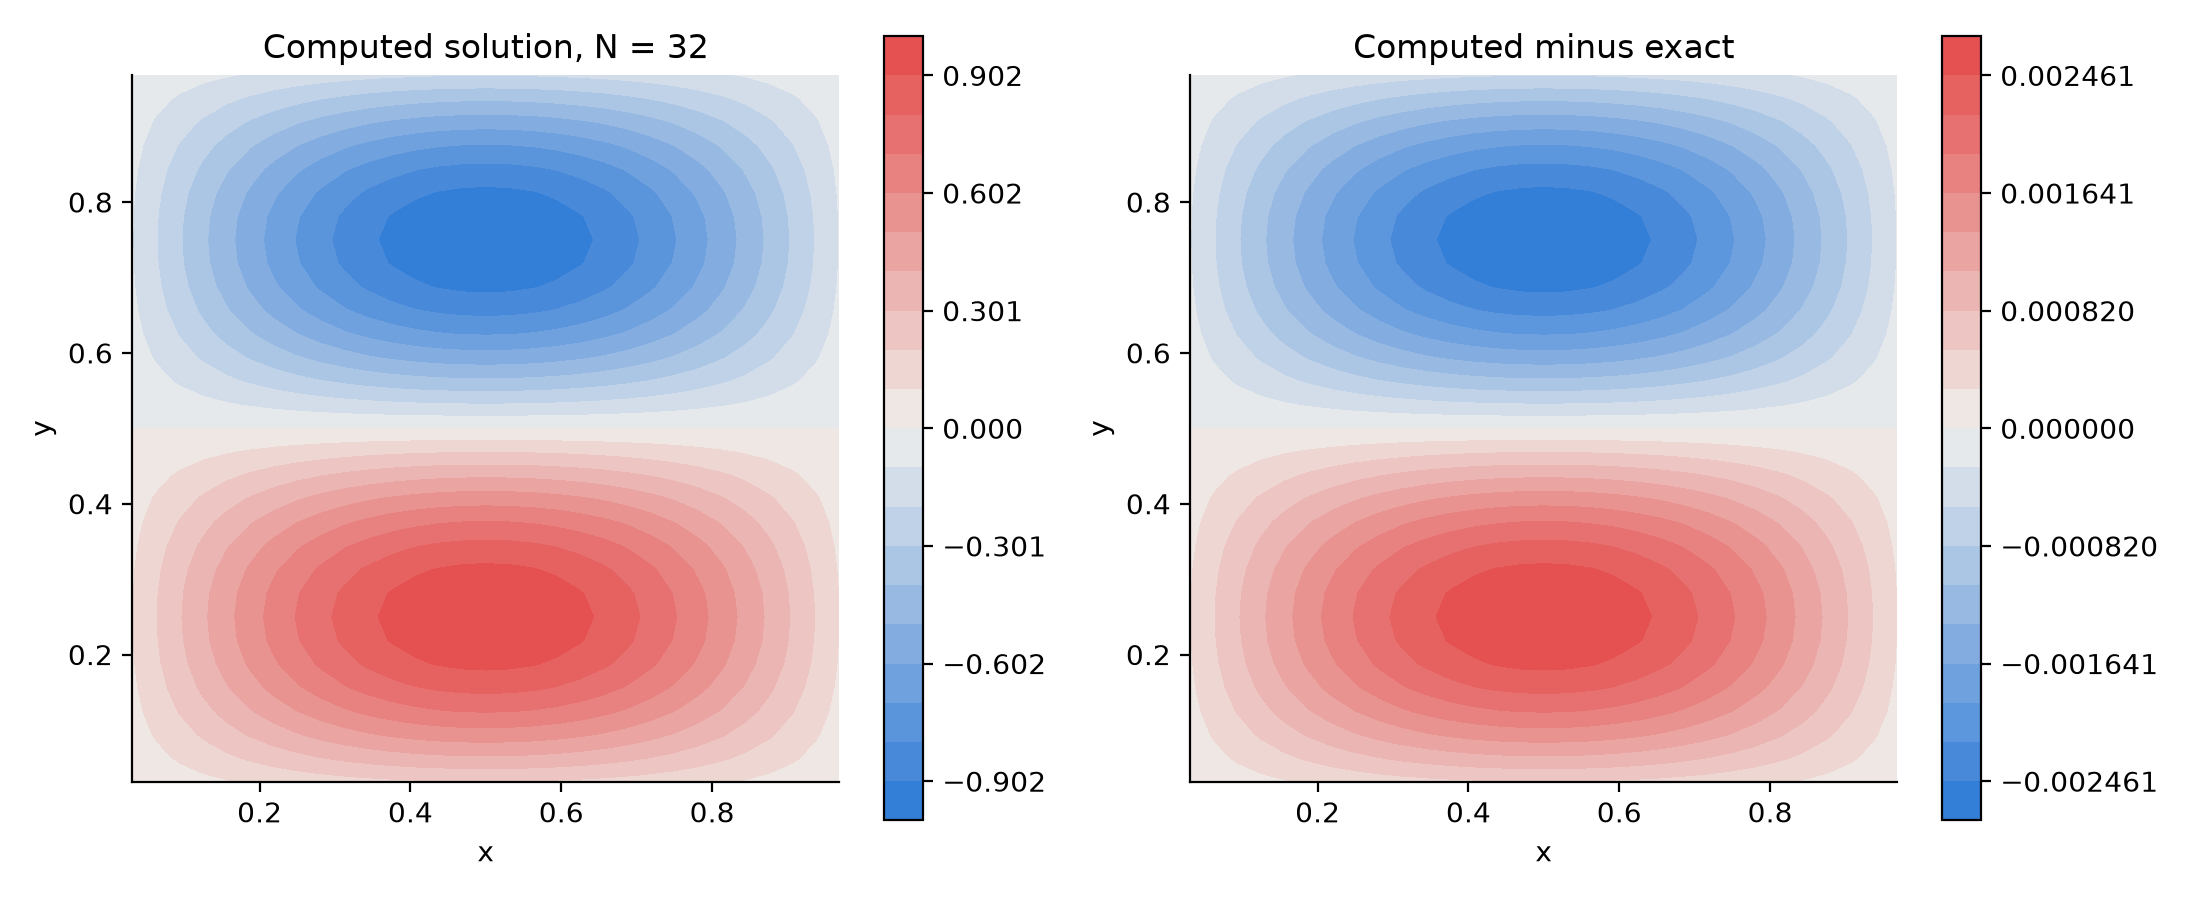
\includegraphics[width=\linewidth]{figures/solution_contour_N32.png}
    \caption{$N = 32$}
    \label{fig:solution-contour-N32}
  \end{subfigure}
  \hfill
  \begin{subfigure}{0.49\textwidth}
    \centering
    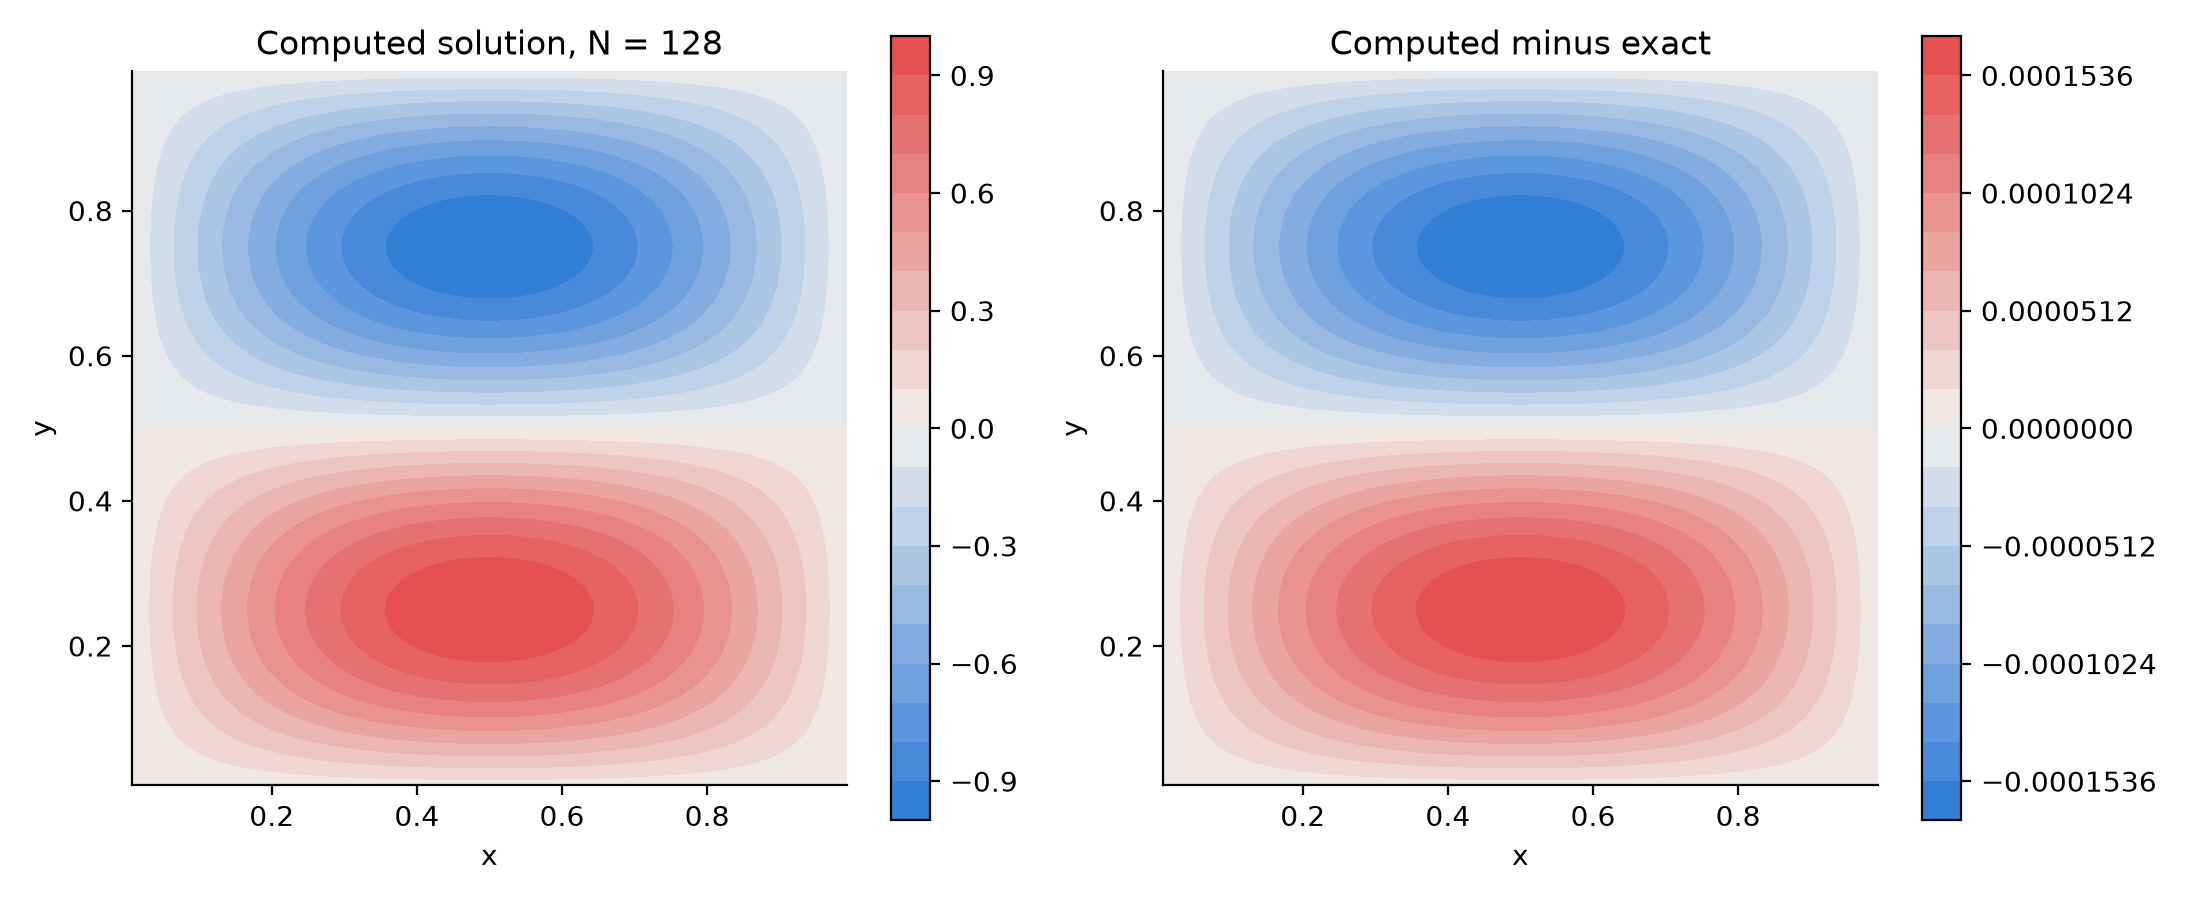
\includegraphics[width=\linewidth]{figures/solution_contour_N128.png}
    \caption{$N = 128$}
    \label{fig:solution-contour-N128}
  \end{subfigure}

  \medskip

  \begin{subfigure}{0.49\textwidth}
    \centering
    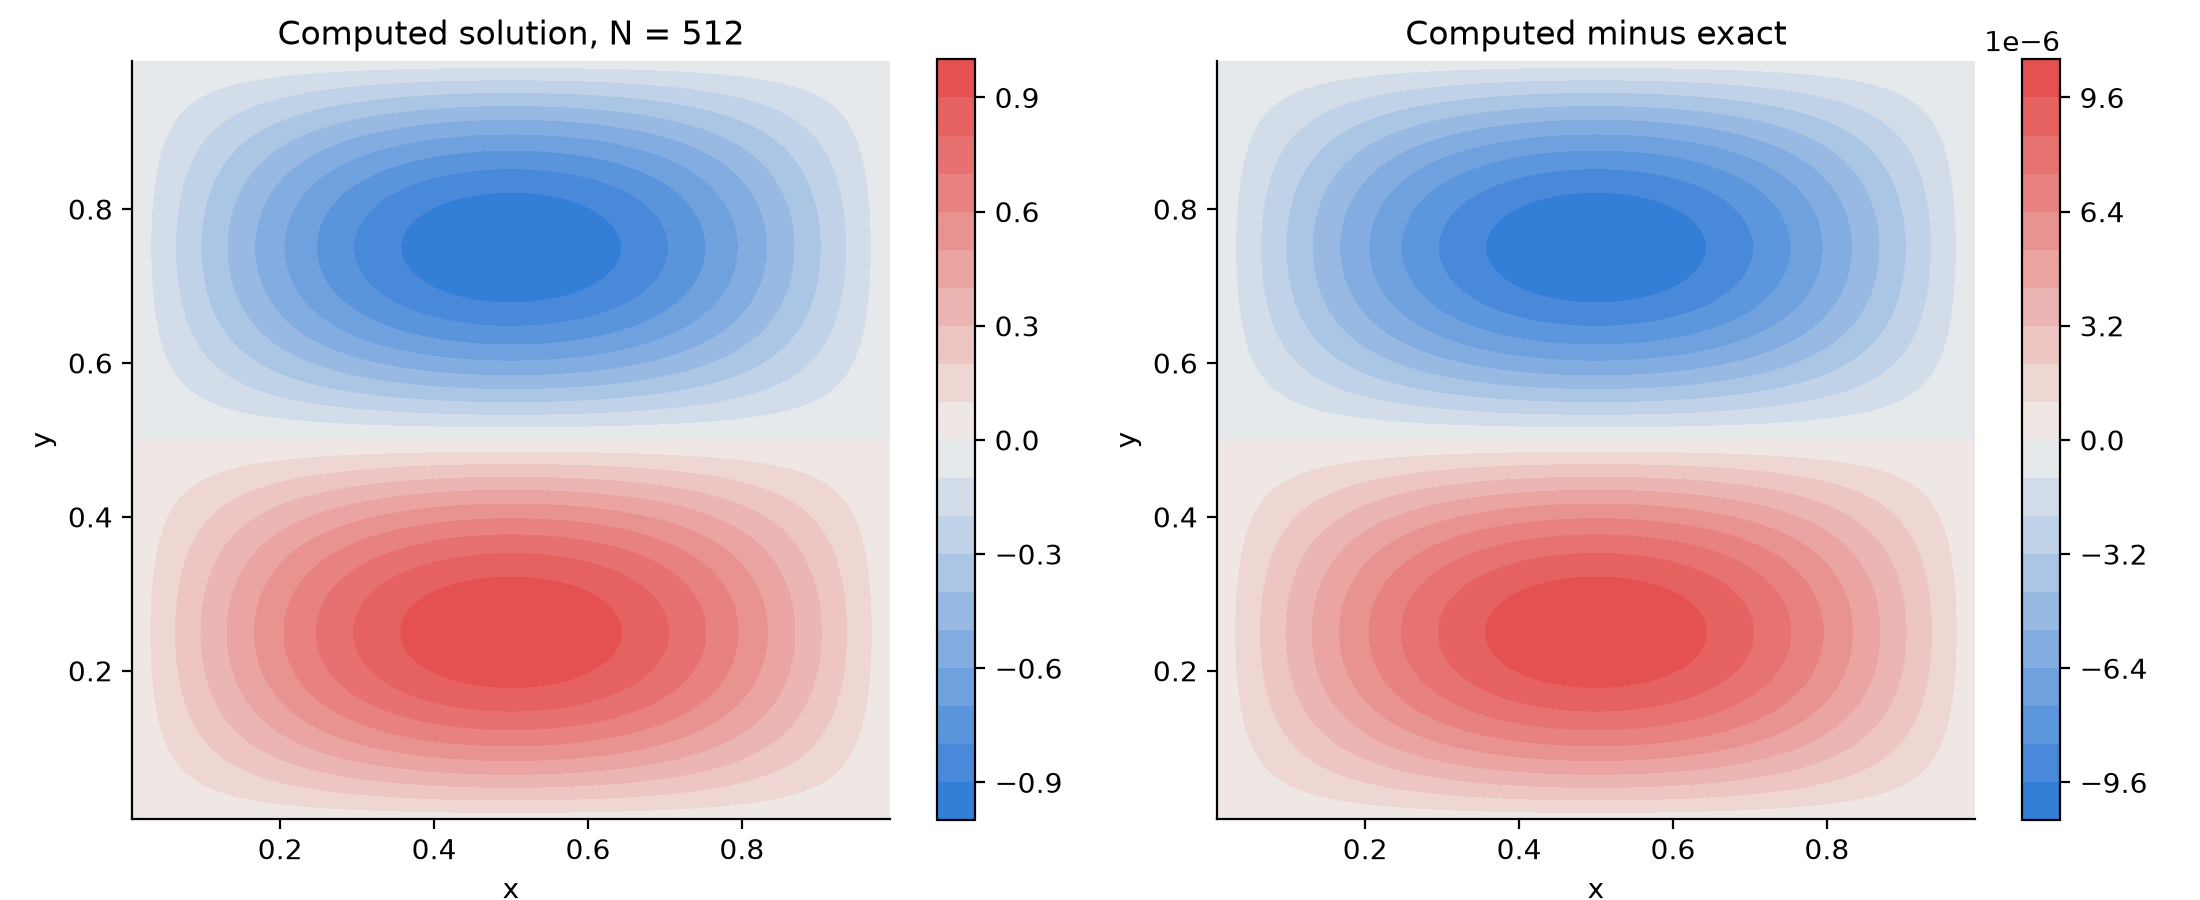
\includegraphics[width=\linewidth]{figures/solution_contour_N512.png}
    \caption{$N = 512$}
    \label{fig:solution-contour-N512}
  \end{subfigure}
  \hfill
  \begin{subfigure}{0.49\textwidth}
    \centering
    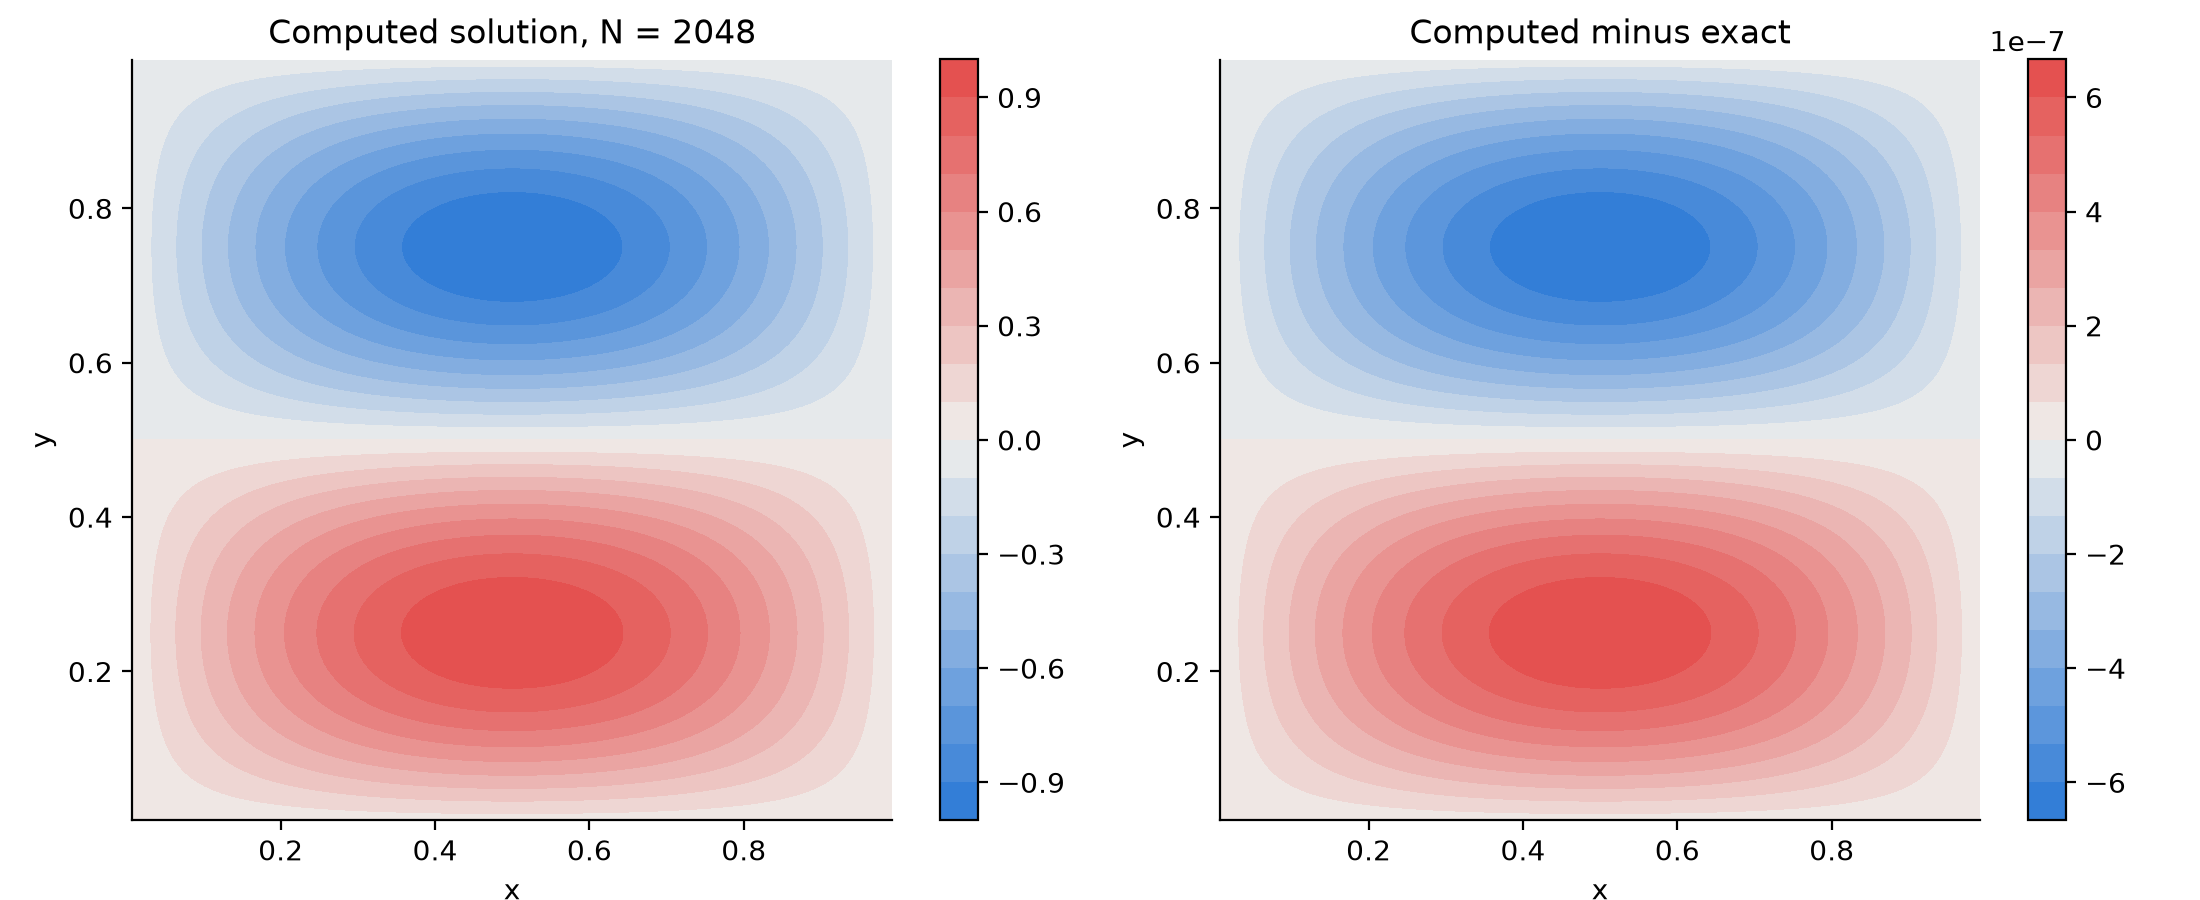
\includegraphics[width=\linewidth]{figures/solution_contour_N2048.png}
    \caption{$N = 2048$}
    \label{fig:solution-contour-N2048}
  \end{subfigure}
  \caption{Computed solution (left panel of each pair) and the difference
    between the computed and exact solutions (right panel) for each grid size
    $N = N_x = N_y$.}
  \label{fig:solution-contours}
\end{figure}

\begin{figure}[htbp]
  \centering
  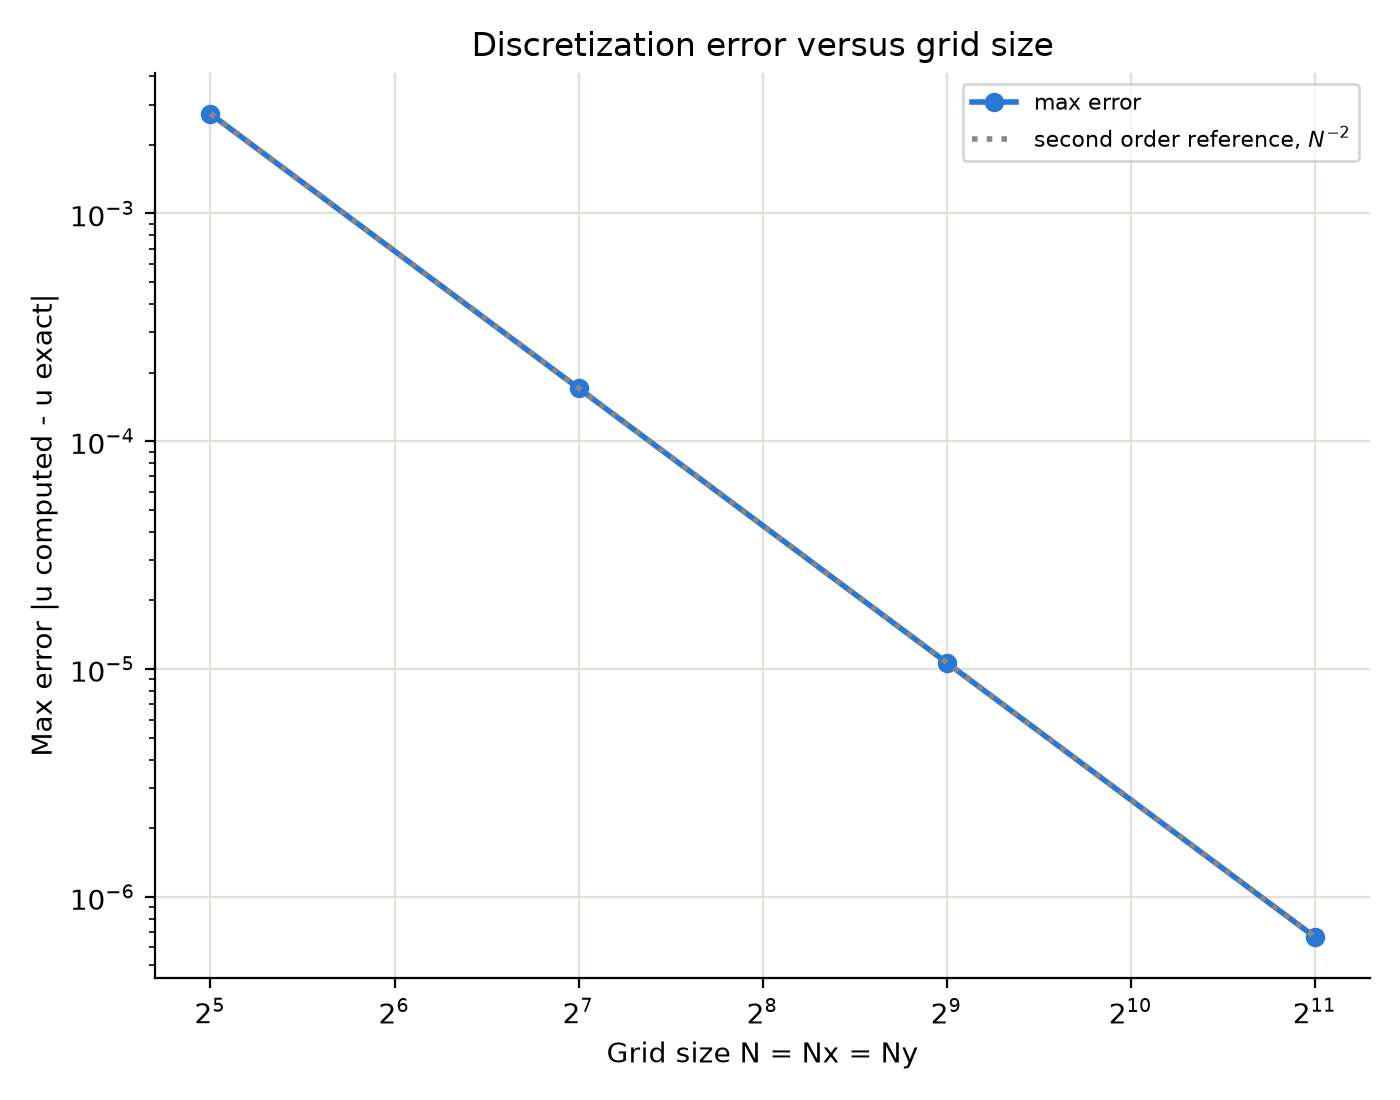
\includegraphics[width=0.45\textwidth]{figures/max_error_versus_grid_size.png}
  \caption{Maximum error of the computed solution versus grid size
    $N = N_x = N_y$, with an $N^{-2}$ reference line.}
  \label{fig:max-error-versus-grid-size}
\end{figure}

\FloatBarrier



% ------------------------------------------------------------ parallel scaling
\subsection{Parallel Scalability}

As indicated by \cref{fig:parallel-scaling}, the benefits of increased number of ranks in a simulation is very much a function of the size of the problem ($N$, in this case).
For example, as indicated by \cref{fig:total-solve-time-versus-ranks}, the maximum compute time for a single problem size is \emph{maximized} when $P=N/2$, which is in some ways counterintuitive, as one would normally expect the compute time to \emph{strictly decrease} with the number of processors.
Interestingly, while the gains in GFLOPS achieved by the increase in processors is clear, the decrease in compute time as a function of processors is marginal at best, given that the total solve time goes from less than a second to less than less than a second\footnote{This is indeed stated with a bit of tongue in cheek.}.
The above results would indicate that gains from parallelism would perhaps be better seen by increasing the problem size further\dots

\begin{figure}[htbp]
  \centering
  \begin{subfigure}{0.49\textwidth}
    \centering
    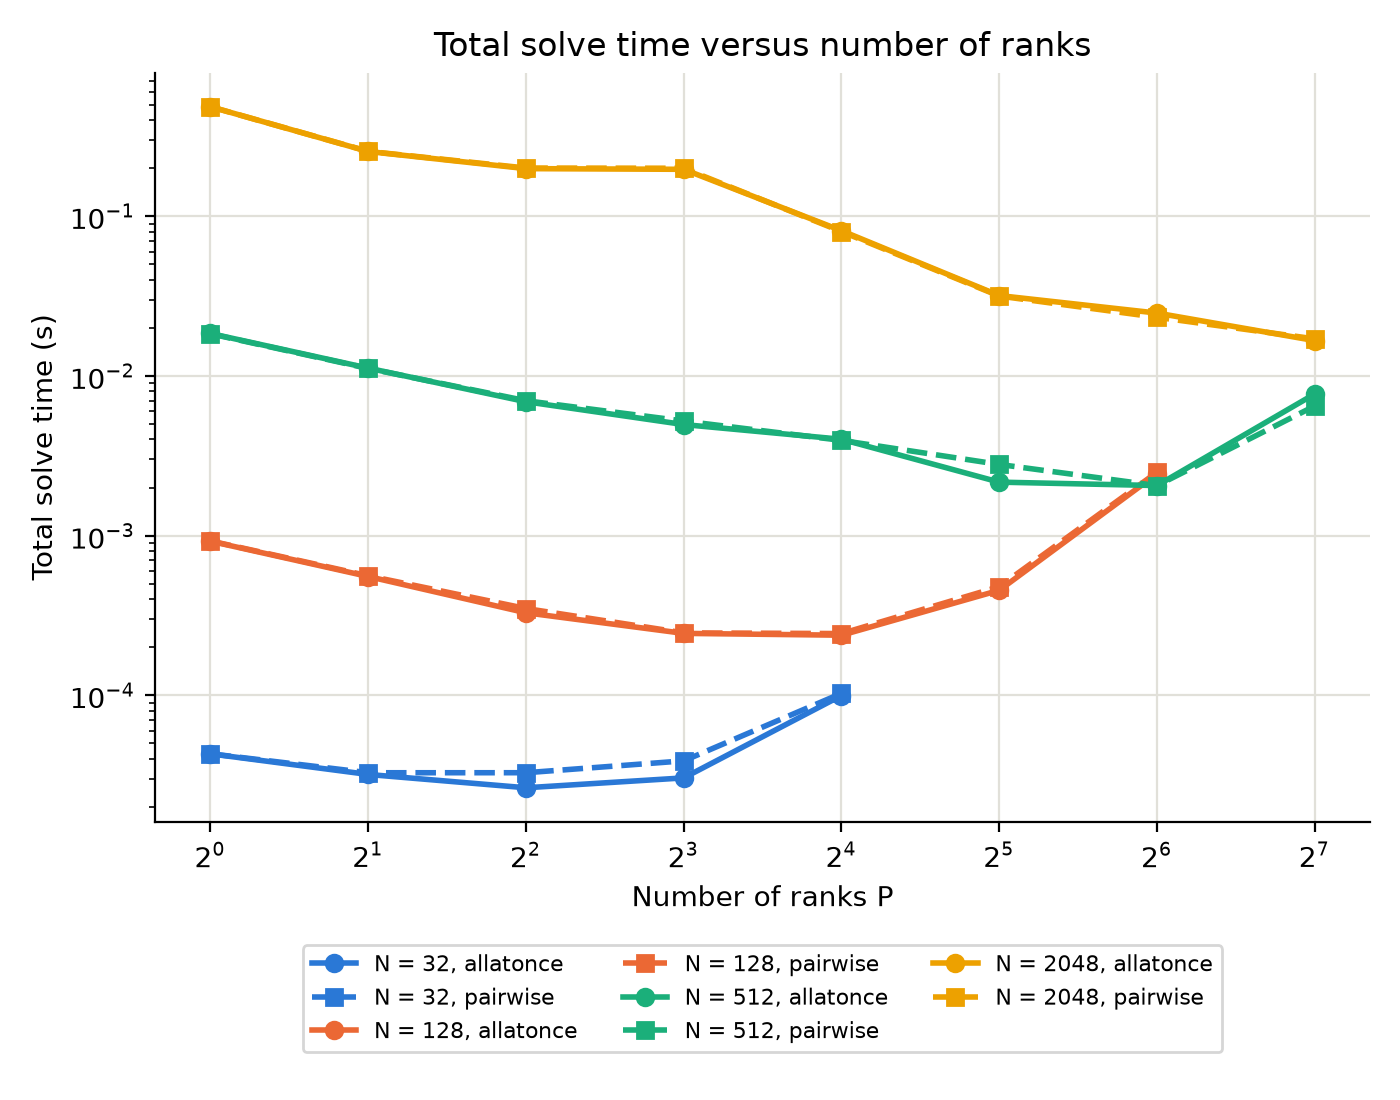
\includegraphics[width=\linewidth]{figures/total_solve_time_versus_ranks.png}
    \caption{Total solve time}
    \label{fig:total-solve-time-versus-ranks}
  \end{subfigure}
  \hfill
  \begin{subfigure}{0.49\textwidth}
    \centering
    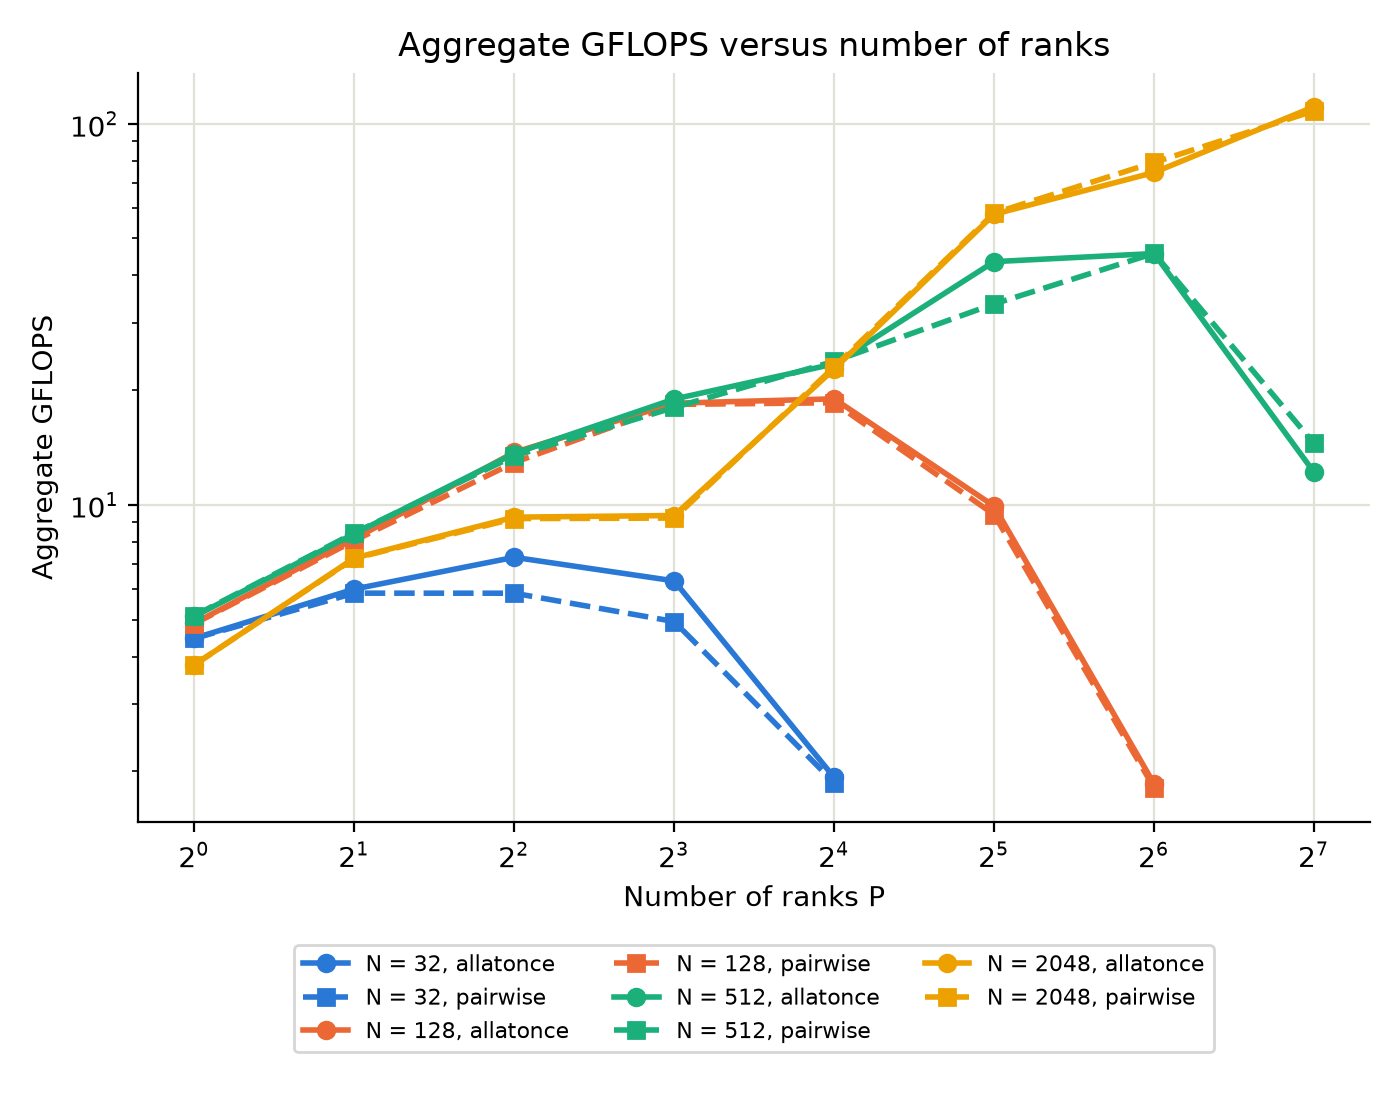
\includegraphics[width=\linewidth]{figures/gflops_versus_ranks.png}
    \caption{Aggregate GFLOPS}
    \label{fig:gflops-versus-ranks}
  \end{subfigure}
  \caption{Total solve time and aggregate GFLOPS versus the number of ranks
    $P$ for each grid size $N$ and both transpose strategies (solid:
    all-at-once, dashed: pairwise).}
  \label{fig:parallel-scaling}
\end{figure}

\FloatBarrier

\subsection{Transpose Comparison}
% TODO: Might be good to add some kind of relative difference plot here for the 2 methods when they are close.

In \cref{fig:fst-and-communication-time} we compare the communication of the two transpose methods across four different values of $n$.
In the plot \cref{fig:fst-time-versus-ranks} shows a largely negligible difference in the two algorithms.
The differences in there performances there vary far less than how each method scales with ranks.
\cref{fig:fst-time-versus-rows-per-rank} tells a similar story.
The plot which shows to a greater degree how these two differ is \cref{fig:communication-time-versus-ranks}.
Here we see the all-at-once largely outperform the the pairwise case.
Notably, the gap is largest at small $n$ where the latency dominates.
It narrows at larger $n$ where this is not the case.



\begin{figure}[htbp]
  \centering
  \begin{subfigure}{0.49\textwidth}
    \centering
    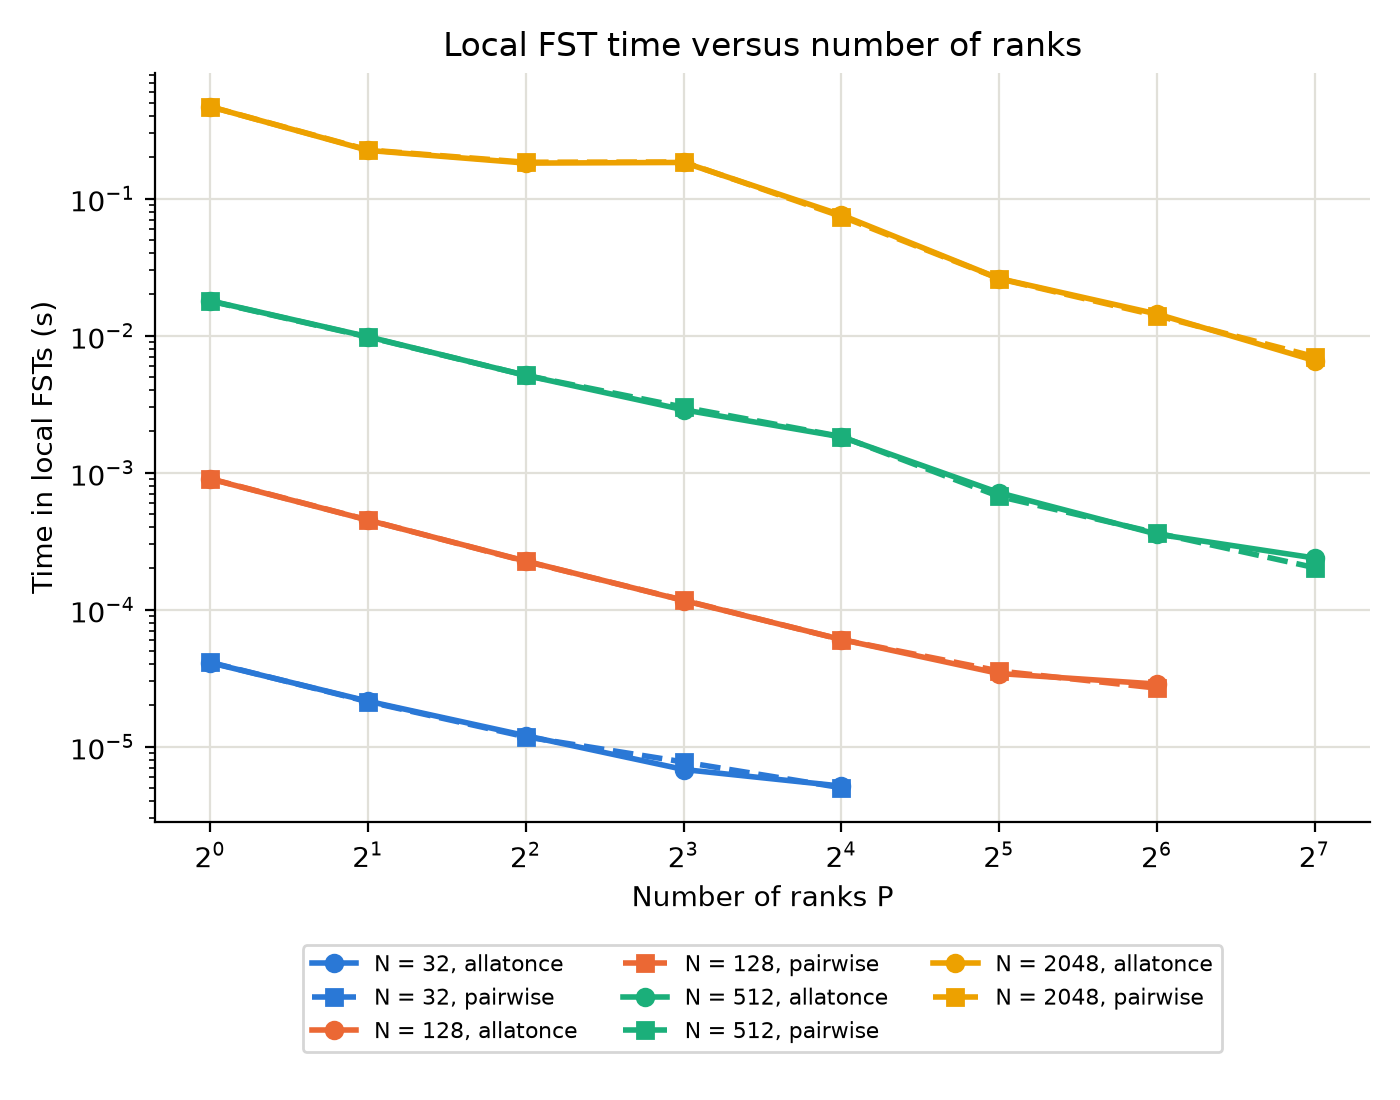
\includegraphics[width=\linewidth]{figures/fst_time_versus_ranks.png}
    \caption{Local FST time versus $P$}
    \label{fig:fst-time-versus-ranks}
  \end{subfigure}
  \hfill
  \begin{subfigure}{0.49\textwidth}
    \centering
    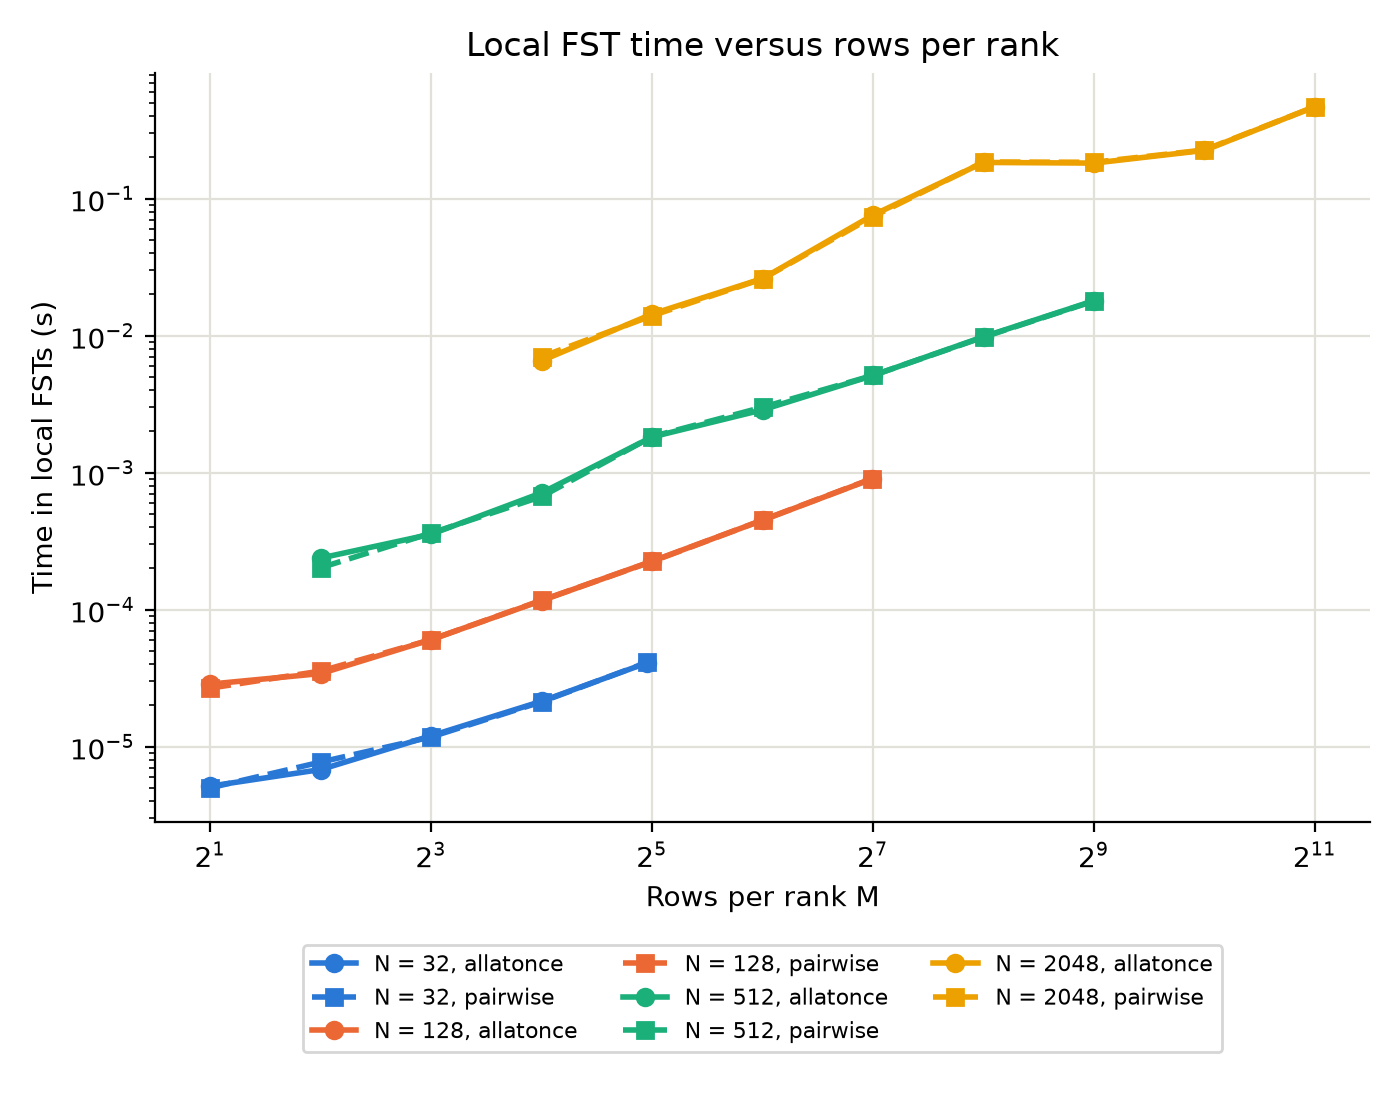
\includegraphics[width=\linewidth]{figures/fst_time_versus_rows_per_rank.png}
    \caption{Local FST time versus $M$}
    \label{fig:fst-time-versus-rows-per-rank}
  \end{subfigure}

  \medskip

  \begin{subfigure}{0.49\textwidth}
    \centering
    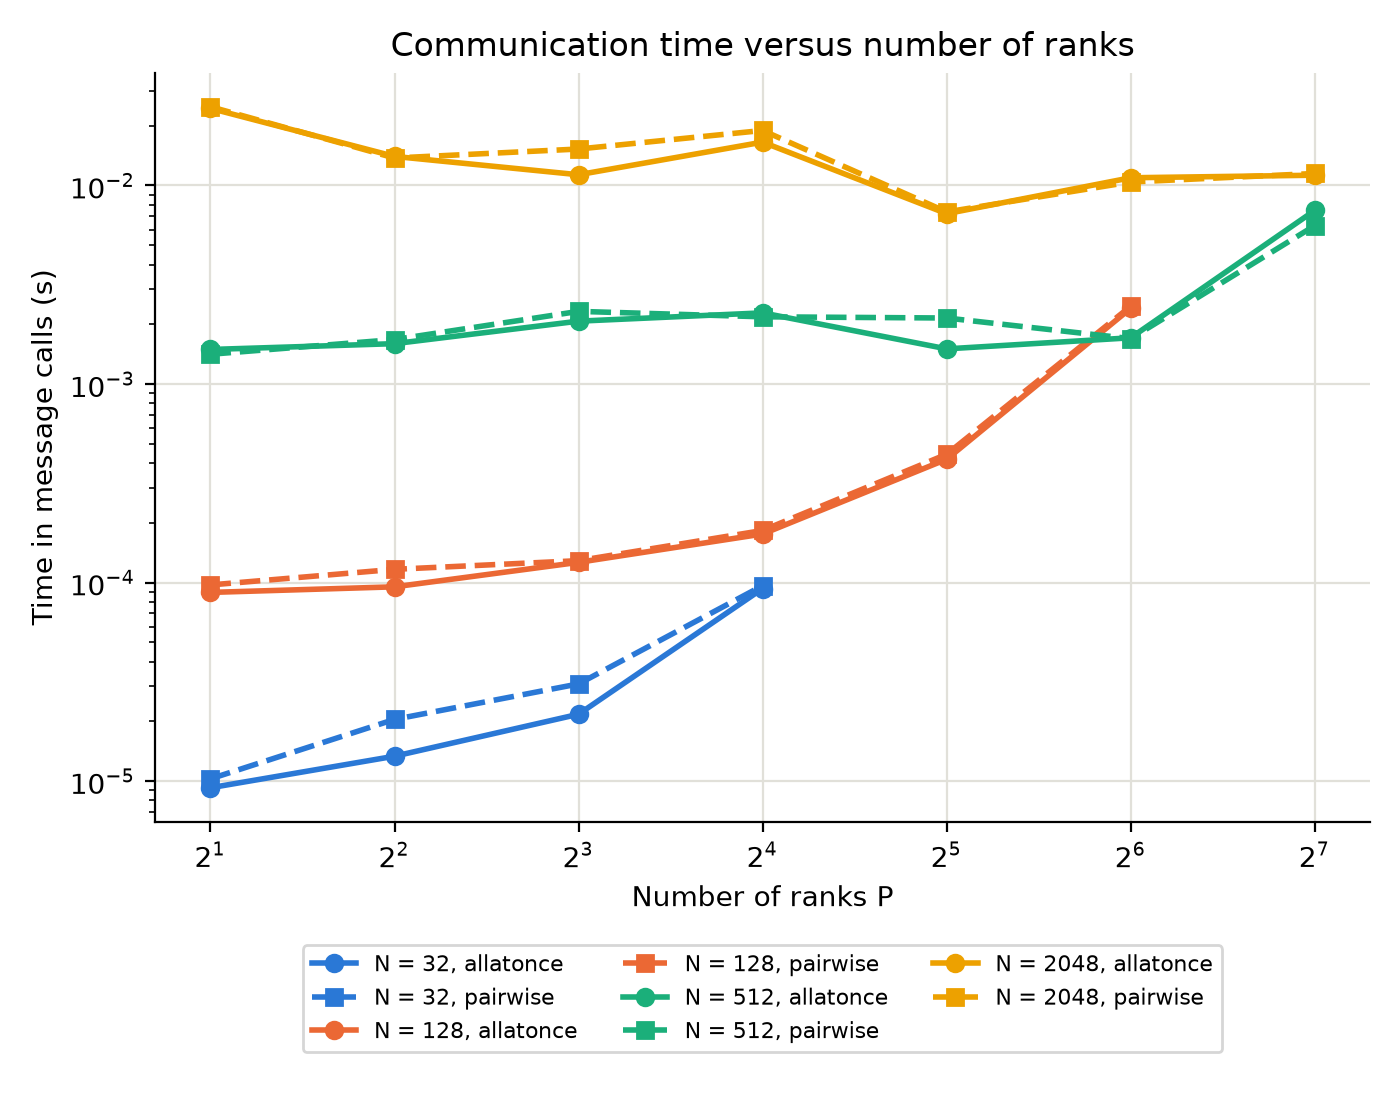
\includegraphics[width=\linewidth]{figures/communication_time_versus_ranks.png}
    \caption{Communication time versus $P$}
    \label{fig:communication-time-versus-ranks}
  \end{subfigure}
  \caption{Time spent in the local fast sine transforms, versus the number of
    ranks $P$ and versus the rows per rank $M$, and time spent in message
    calls versus $P$, for each grid size $N$ and both transpose strategies.}
  \label{fig:fst-and-communication-time}
\end{figure}

\FloatBarrier




\pagebreak
% --------------------------------------------- single core and communication
\subsection{Single Core}
\begin{figure}[htbp]
  \centering
  \begin{subfigure}{0.49\textwidth}
    \centering
    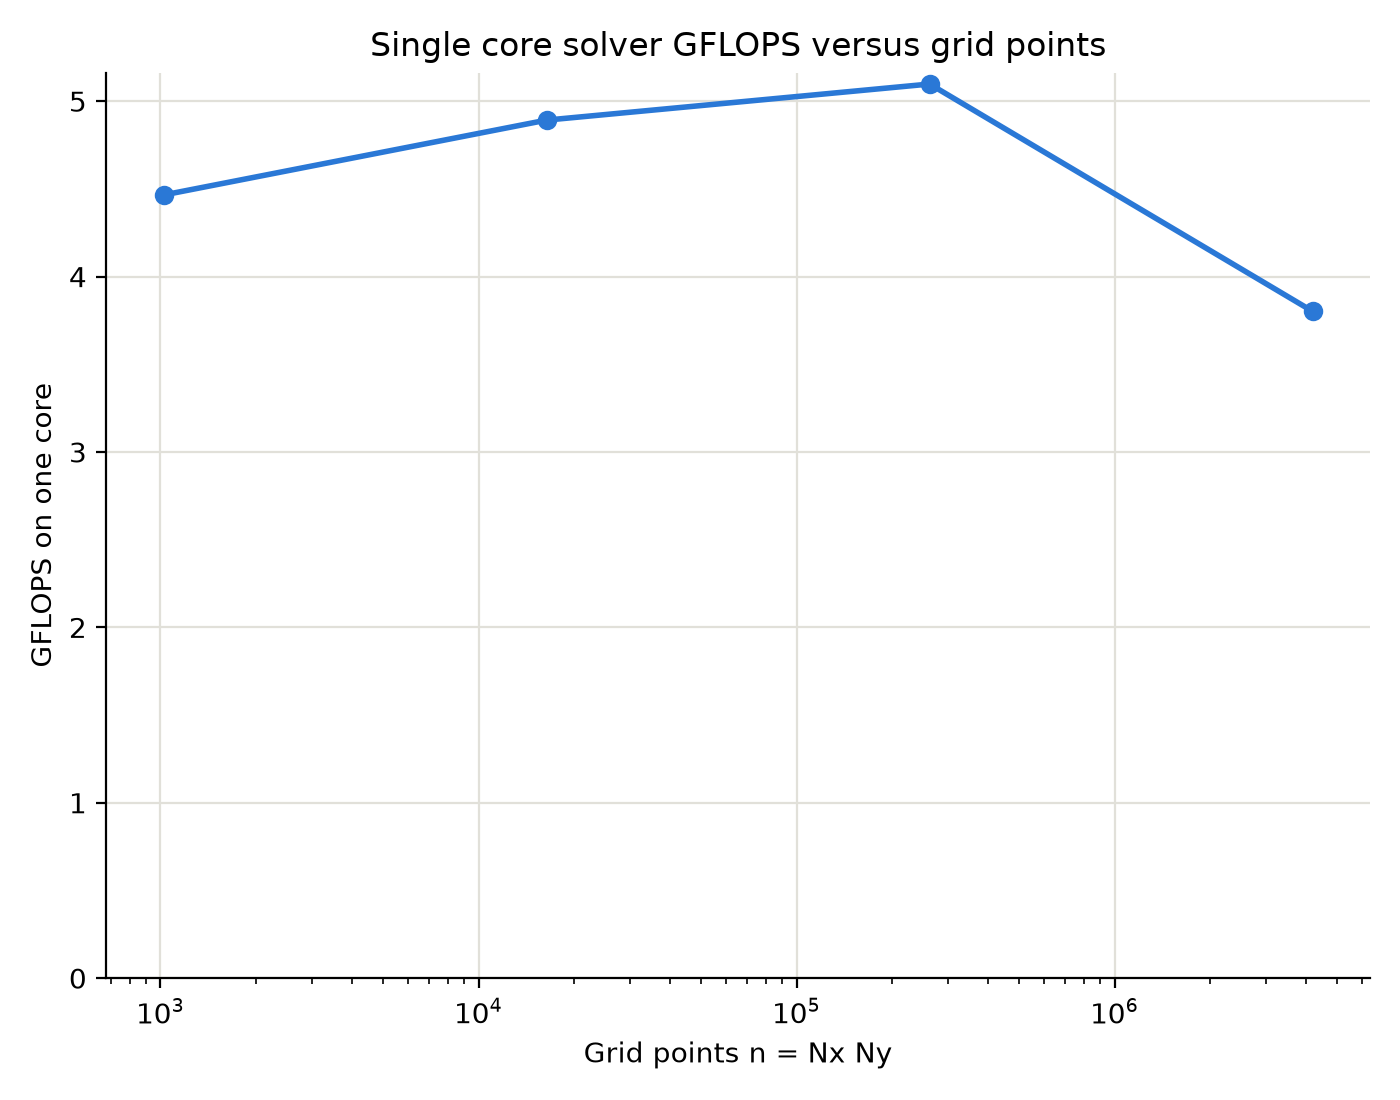
\includegraphics[width=\linewidth]{figures/single_core_gflops_versus_grid_points.png}
    \caption{Full solve versus grid points $n = N_x N_y$}
    \label{fig:single-core-gflops-versus-grid-points}
  \end{subfigure}
  \hfill
  \begin{subfigure}{0.49\textwidth}
    \centering
    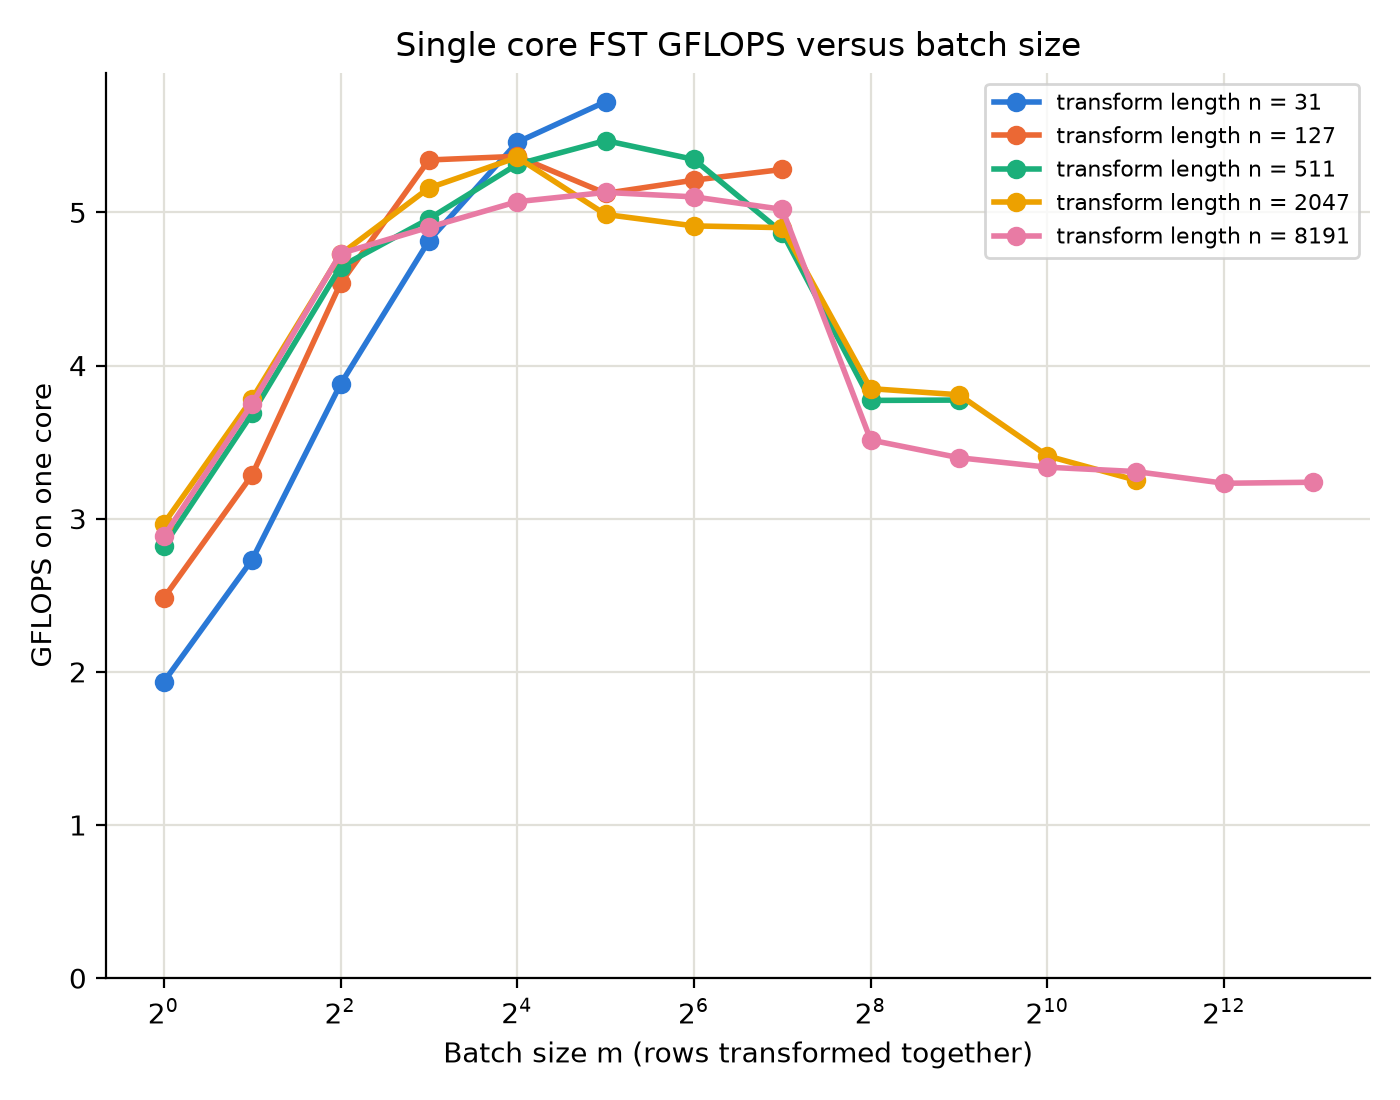
\includegraphics[width=\linewidth]{figures/single_core_fst_gflops_versus_batch_size.png}
    \caption{Batched FST versus batch size $m$}
    \label{fig:single-core-fst-gflops-versus-batch-size}
  \end{subfigure}
  \caption{Single-core GFLOPS of the full Poisson solve and of the batched
    fast sine transform alone, the latter for each transform length $n$.}
  \label{fig:single-core-performance}
\end{figure}


\FloatBarrier

\pagebreak

A ping-pong test was performed, with results reported in \cref{fig:pingpong-time-versus-message-size}.
As expected, the internode message hovers about the same distance away from the intranode messaging, showing how the message communication asymptotically approaches a fixed value of time for jumping a message across nodes.

\begin{figure}[htbp]
  \centering
  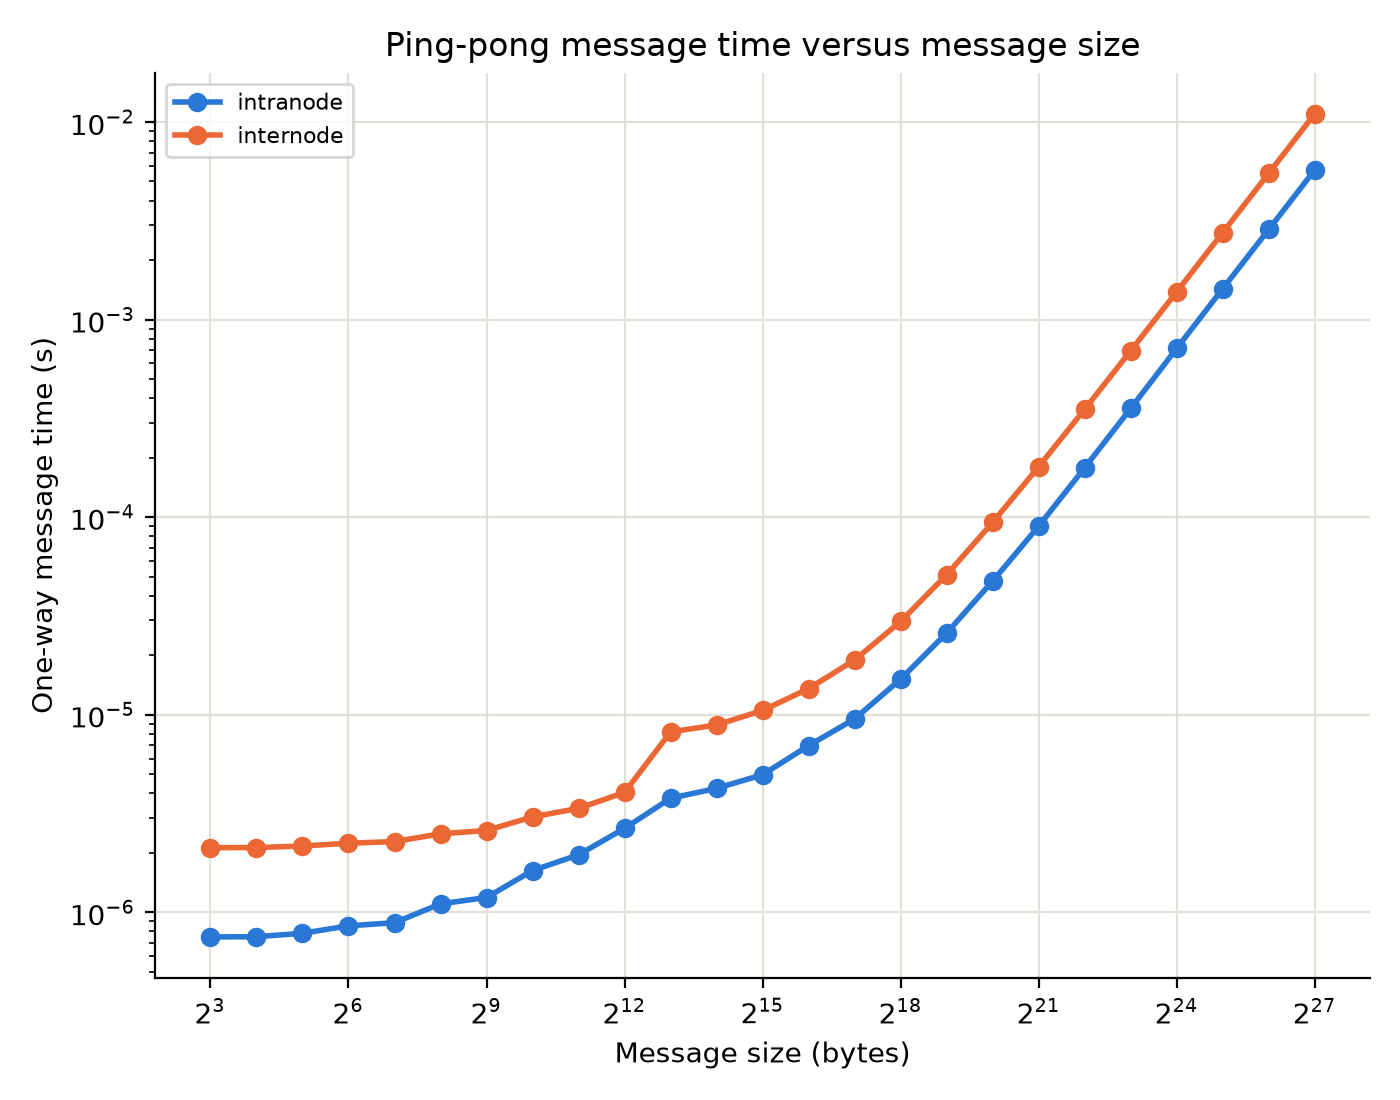
\includegraphics[width=0.6\textwidth]{figures/pingpong_time_versus_message_size.png}
  \caption{One-way point-to-point message time versus message size from the
    ping-pong test, with both ranks on one node (intranode) and on two
    different nodes (internode).}
  \label{fig:pingpong-time-versus-message-size}
\end{figure}

\FloatBarrier

% ------------------------------------------------------- model and efficiency

\begin{figure}[htbp]
  \centering
  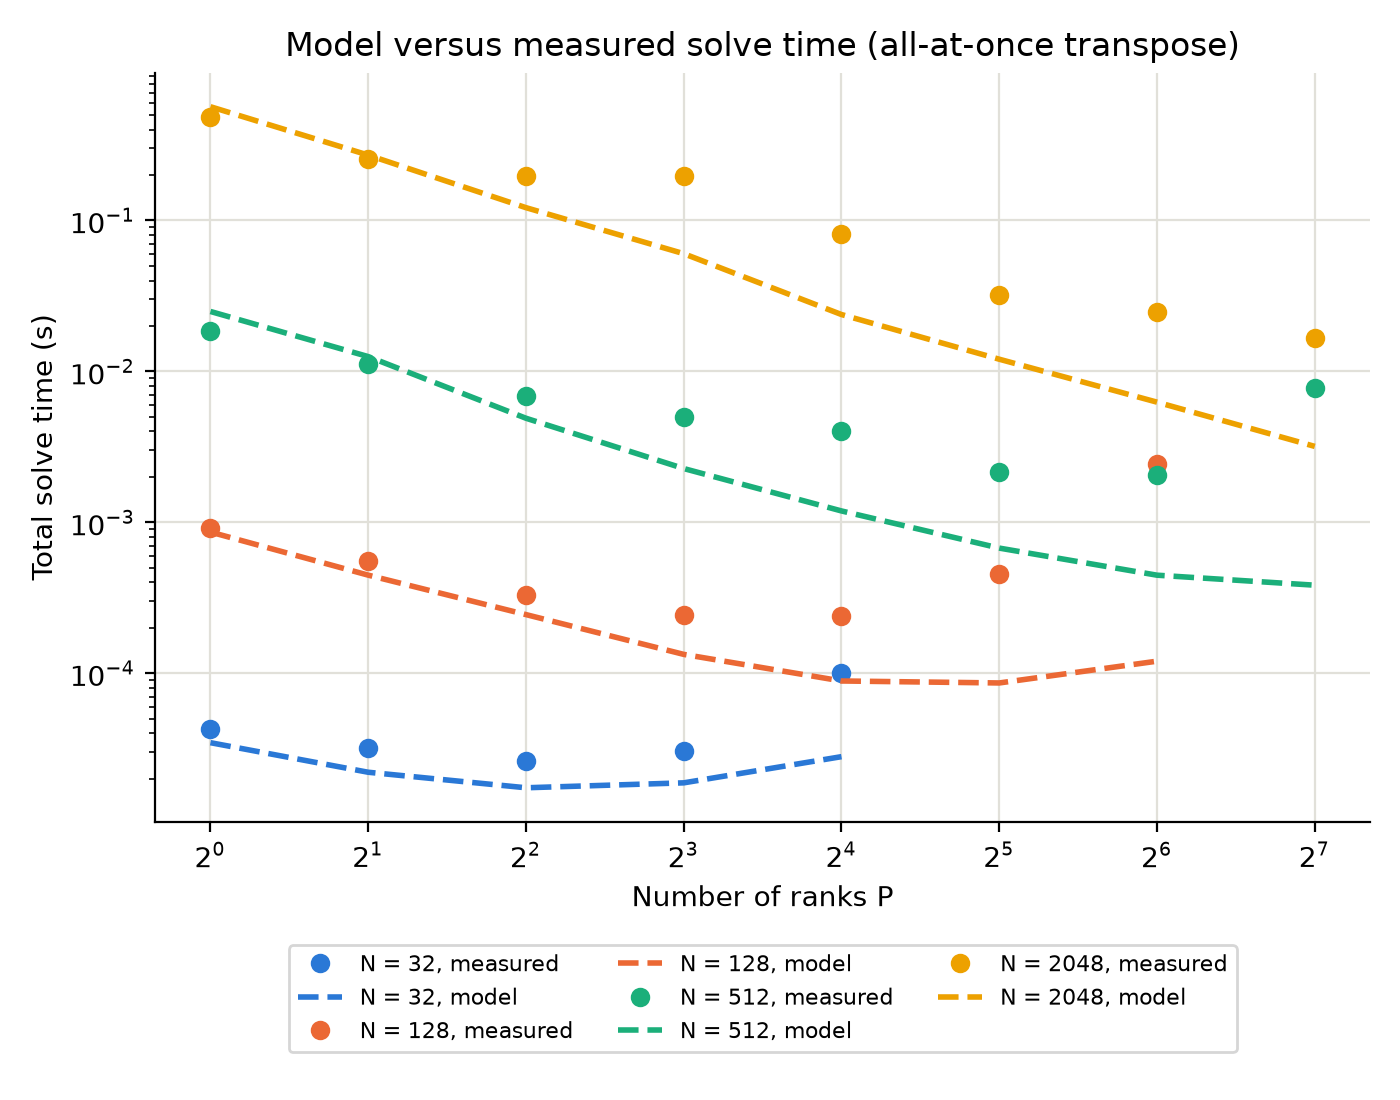
\includegraphics[width=0.6\textwidth]{figures/model_versus_measured_solve_time.png}
  \caption{Measured total solve time (markers) and the performance model
    (dashed lines) versus the number of ranks $P$ for each grid size $N$,
    all-at-once transpose.}
  \label{fig:model-versus-measured-solve-time}
\end{figure}

The compute time per rank for $P$ total ranks is:
\begin{equation}
  T_P=\text{computer time per rank}+\text{communication}
\end{equation}
with the ideal being:
\begin{equation}
  \label{eq:ideal_tp}
  T_{P,\text{ideal}}=\frac{T_1}{P}.
\end{equation}
\Cref{eq:ideal_tp} shows that if everything goes our way, we should see a drop off in FST compute time by a factor of two with every doubling of the number of processors.
While this is evidently true for $N=32,128$, the same can certainly \emph{not} be said for $N=2048$ (see \cref{fig:parallel-efficiency-versus-points-per-rank}).
Indeed, for $N=2048$, we observe a steep drop off in efficiency (notably the number of GFLOPS) as the number of processors increases even though the work required per processor continues to decrease.
A possible explanation for this is that the memory required for each processor exceeds the private local cache, meaning memory resources are being accessed from a shared cache, leading to memory contention.
This would explain why we eventually see a ``bump'' back up in efficiency -- the required memory is now small enough to be localized, removing the resource fight.

As indicated by \cref{tab:efficiency-80}, none of the values passed for $N$ yielded exactly 80\% efficiency.
However, values for these have been interpolated between neighboring points and reported.
Performance limitations are dependent on multiple factors, but notably the problem size.
For $N=32,128$, performance is limited simply by the communication overhead.
However, for $N=2048$, performance could limited by memory access since we are no longer able to store the necessary data for processes in a rank in a local private cache until the number of processors is large enough to fit the split data into small enough chunks.

\begin{table}
  \centering
  \begin{adjustbox}{max width=\textwidth, max totalheight=0.95\textheight}
    \begin{tabular}{lllllllllll}
      \toprule
      P   & Nx   & Ny   & mode      & M    & t\_total & t\_fst   & t\_transpose & t\_comm  & gflops & error    \\
      \midrule
      1   & 128  & 128  & allatonce & 127  & 9.23E-04 & 9.00E-04 & 2.29E-05     & 1.60E-07 & 4.89   & 1.71E-04 \\
      1   & 128  & 128  & pairwise  & 127  & 9.27E-04 & 9.03E-04 & 2.30E-05     & 0.00E+00 & 4.87   & 1.71E-04 \\
      1   & 2048 & 2048 & allatonce & 2047 & 4.85E-01 & 4.69E-01 & 1.63E-02     & 8.01E-07 & 3.80   & 6.67E-07 \\
      1   & 2048 & 2048 & pairwise  & 2047 & 4.85E-01 & 4.68E-01 & 1.63E-02     & 0.00E+00 & 3.80   & 6.67E-07 \\
      1   & 32   & 32   & allatonce & 31   & 4.30E-05 & 4.10E-05 & 1.81E-06     & 1.30E-07 & 4.47   & 2.73E-03 \\
      1   & 32   & 32   & pairwise  & 31   & 4.31E-05 & 4.13E-05 & 1.58E-06     & 0.00E+00 & 4.46   & 2.73E-03 \\
      1   & 512  & 512  & allatonce & 511  & 1.84E-02 & 1.80E-02 & 4.85E-04     & 1.80E-07 & 5.10   & 1.07E-05 \\
      1   & 512  & 512  & pairwise  & 511  & 1.84E-02 & 1.79E-02 & 4.85E-04     & 0.00E+00 & 5.12   & 1.07E-05 \\
      2   & 128  & 128  & allatonce & 64   & 5.55E-04 & 4.50E-04 & 1.07E-04     & 8.93E-05 & 8.14   & 1.71E-04 \\
      2   & 128  & 128  & pairwise  & 64   & 5.61E-04 & 4.51E-04 & 1.14E-04     & 9.74E-05 & 8.05   & 1.71E-04 \\
      2   & 2048 & 2048 & allatonce & 1024 & 2.54E-01 & 2.25E-01 & 3.20E-02     & 2.44E-02 & 7.25   & 6.67E-07 \\
      2   & 2048 & 2048 & pairwise  & 1024 & 2.55E-01 & 2.27E-01 & 3.20E-02     & 2.49E-02 & 7.24   & 6.67E-07 \\
      2   & 32   & 32   & allatonce & 16   & 3.20E-05 & 2.15E-05 & 1.03E-05     & 9.27E-06 & 6.01   & 2.73E-03 \\
      2   & 32   & 32   & pairwise  & 16   & 3.28E-05 & 2.13E-05 & 1.13E-05     & 1.03E-05 & 5.86   & 2.73E-03 \\
      2   & 512  & 512  & allatonce & 256  & 1.12E-02 & 9.82E-03 & 1.77E-03     & 1.49E-03 & 8.40   & 1.07E-05 \\
      2   & 512  & 512  & pairwise  & 256  & 1.11E-02 & 9.77E-03 & 1.72E-03     & 1.41E-03 & 8.44   & 1.07E-05 \\
      4   & 128  & 128  & allatonce & 32   & 3.29E-04 & 2.26E-04 & 1.05E-04     & 9.53E-05 & 13.73  & 1.71E-04 \\
      4   & 128  & 128  & pairwise  & 32   & 3.50E-04 & 2.25E-04 & 1.25E-04     & 1.17E-04 & 12.91  & 1.71E-04 \\
      4   & 2048 & 2048 & allatonce & 512  & 1.99E-01 & 1.82E-01 & 1.89E-02     & 1.40E-02 & 9.28   & 6.67E-07 \\
      4   & 2048 & 2048 & pairwise  & 512  & 2.00E-01 & 1.84E-01 & 2.10E-02     & 1.38E-02 & 9.20   & 6.67E-07 \\
      4   & 32   & 32   & allatonce & 8    & 2.64E-05 & 1.20E-05 & 1.44E-05     & 1.34E-05 & 7.28   & 2.73E-03 \\
      4   & 32   & 32   & pairwise  & 8    & 3.28E-05 & 1.18E-05 & 2.11E-05     & 2.05E-05 & 5.86   & 2.73E-03 \\
      4   & 512  & 512  & allatonce & 128  & 6.90E-03 & 5.12E-03 & 1.81E-03     & 1.60E-03 & 13.63  & 1.07E-05 \\
      4   & 512  & 512  & pairwise  & 128  & 7.00E-03 & 5.13E-03 & 1.92E-03     & 1.68E-03 & 13.44  & 1.07E-05 \\
      8   & 128  & 128  & allatonce & 16   & 2.44E-04 & 1.17E-04 & 1.31E-04     & 1.27E-04 & 18.48  & 1.71E-04 \\
      8   & 128  & 128  & pairwise  & 16   & 2.46E-04 & 1.17E-04 & 1.33E-04     & 1.29E-04 & 18.34  & 1.71E-04 \\
      8   & 2048 & 2048 & allatonce & 256  & 1.97E-01 & 1.84E-01 & 1.59E-02     & 1.13E-02 & 9.38   & 6.67E-07 \\
      8   & 2048 & 2048 & pairwise  & 256  & 2.00E-01 & 1.85E-01 & 1.91E-02     & 1.53E-02 & 9.23   & 6.67E-07 \\
      8   & 32   & 32   & allatonce & 4    & 3.04E-05 & 6.82E-06 & 2.37E-05     & 2.17E-05 & 6.32   & 2.73E-03 \\
      8   & 32   & 32   & pairwise  & 4    & 3.89E-05 & 7.74E-06 & 3.17E-05     & 3.09E-05 & 4.94   & 2.73E-03 \\
      8   & 512  & 512  & allatonce & 64   & 4.96E-03 & 2.88E-03 & 2.16E-03     & 2.07E-03 & 18.95  & 1.07E-05 \\
      8   & 512  & 512  & pairwise  & 64   & 5.22E-03 & 3.01E-03 & 2.42E-03     & 2.32E-03 & 18.01  & 1.07E-05 \\
      16  & 128  & 128  & allatonce & 8    & 2.38E-04 & 6.06E-05 & 1.78E-04     & 1.76E-04 & 18.97  & 1.71E-04 \\
      16  & 128  & 128  & pairwise  & 8    & 2.44E-04 & 6.05E-05 & 1.86E-04     & 1.83E-04 & 18.53  & 1.71E-04 \\
      16  & 2048 & 2048 & allatonce & 128  & 8.12E-02 & 7.59E-02 & 1.88E-02     & 1.65E-02 & 22.72  & 6.67E-07 \\
      16  & 2048 & 2048 & pairwise  & 128  & 8.02E-02 & 7.40E-02 & 2.09E-02     & 1.89E-02 & 23.00  & 6.67E-07 \\
      16  & 32   & 32   & allatonce & 2    & 9.98E-05 & 5.16E-06 & 9.45E-05     & 9.34E-05 & 1.93   & 2.73E-03 \\
      16  & 32   & 32   & pairwise  & 2    & 1.03E-04 & 5.02E-06 & 9.80E-05     & 9.66E-05 & 1.87   & 2.73E-03 \\
      16  & 512  & 512  & allatonce & 32   & 4.01E-03 & 1.82E-03 & 2.35E-03     & 2.28E-03 & 23.43  & 1.07E-05 \\
      16  & 512  & 512  & pairwise  & 32   & 3.95E-03 & 1.84E-03 & 2.22E-03     & 2.18E-03 & 23.81  & 1.07E-05 \\
      32  & 128  & 128  & allatonce & 4    & 4.55E-04 & 3.42E-05 & 4.22E-04     & 4.18E-04 & 9.93   & 1.71E-04 \\
      32  & 128  & 128  & pairwise  & 4    & 4.79E-04 & 3.57E-05 & 4.46E-04     & 4.43E-04 & 9.43   & 1.71E-04 \\
      32  & 2048 & 2048 & allatonce & 64   & 3.19E-02 & 2.61E-02 & 8.87E-03     & 7.21E-03 & 57.86  & 6.67E-07 \\
      32  & 2048 & 2048 & pairwise  & 64   & 3.16E-02 & 2.60E-02 & 8.39E-03     & 7.36E-03 & 58.27  & 6.67E-07 \\
      32  & 512  & 512  & allatonce & 16   & 2.16E-03 & 7.14E-04 & 1.52E-03     & 1.50E-03 & 43.46  & 1.07E-05 \\
      32  & 512  & 512  & pairwise  & 16   & 2.79E-03 & 6.70E-04 & 2.17E-03     & 2.15E-03 & 33.66  & 1.07E-05 \\
      64  & 128  & 128  & allatonce & 2    & 2.44E-03 & 2.87E-05 & 2.41E-03     & 2.41E-03 & 1.85   & 1.71E-04 \\
      64  & 128  & 128  & pairwise  & 2    & 2.50E-03 & 2.68E-05 & 2.47E-03     & 2.47E-03 & 1.81   & 1.71E-04 \\
      64  & 2048 & 2048 & allatonce & 32   & 2.48E-02 & 1.44E-02 & 1.17E-02     & 1.09E-02 & 74.48  & 6.67E-07 \\
      64  & 2048 & 2048 & pairwise  & 32   & 2.33E-02 & 1.40E-02 & 1.06E-02     & 1.04E-02 & 79.16  & 6.67E-07 \\
      64  & 512  & 512  & allatonce & 8    & 2.06E-03 & 3.56E-04 & 1.73E-03     & 1.71E-03 & 45.65  & 1.07E-05 \\
      64  & 512  & 512  & pairwise  & 8    & 2.06E-03 & 3.63E-04 & 1.71E-03     & 1.69E-03 & 45.69  & 1.07E-05 \\
      128 & 2048 & 2048 & allatonce & 16   & 1.66E-02 & 6.57E-03 & 1.14E-02     & 1.13E-02 & 110.81 & 6.67E-07 \\
      128 & 2048 & 2048 & pairwise  & 16   & 1.71E-02 & 7.02E-03 & 1.16E-02     & 1.15E-02 & 108.05 & 6.67E-07 \\
      128 & 512  & 512  & allatonce & 4    & 7.72E-03 & 2.38E-04 & 7.50E-03     & 7.49E-03 & 12.18  & 1.07E-05 \\
      128 & 512  & 512  & pairwise  & 4    & 6.49E-03 & 2.03E-04 & 6.29E-03     & 6.28E-03 & 14.49  & 1.07E-05 \\
      \bottomrule
    \end{tabular}
  \end{adjustbox}
  \caption{Timings for FST and transpositions. Also reporting alongside the number of GFLOPS and the error.}
  \caption{tab:timings}
\end{table}

\begin{table}
  \centering
  \begin{adjustbox}{max width=\textwidth, max totalheight=0.95\textheight}
    \begin{tabular}{lllllllll}
      \toprule
      P   & Nx   & Ny   & mode      & M    & FST \%  & Transpose \% & Communication \% & gflops \\
      \midrule
      1   & 128  & 128  & allatonce & 127  & 97.48\% & 2.48\%       & 0.02\%           & 4.89   \\
      1   & 128  & 128  & pairwise  & 127  & 97.49\% & 2.48\%       & 0.00\%           & 4.87   \\
      1   & 2048 & 2048 & allatonce & 2047 & 96.64\% & 3.35\%       & 0.00\%           & 3.80   \\
      1   & 2048 & 2048 & pairwise  & 2047 & 96.65\% & 3.35\%       & 0.00\%           & 3.80   \\
      1   & 32   & 32   & allatonce & 31   & 95.25\% & 4.21\%       & 0.30\%           & 4.47   \\
      1   & 32   & 32   & pairwise  & 31   & 95.79\% & 3.67\%       & 0.00\%           & 4.46   \\
      1   & 512  & 512  & allatonce & 511  & 97.37\% & 2.63\%       & 0.00\%           & 5.10   \\
      1   & 512  & 512  & pairwise  & 511  & 97.36\% & 2.64\%       & 0.00\%           & 5.12   \\
      2   & 128  & 128  & allatonce & 64   & 81.13\% & 19.34\%      & 16.09\%          & 8.14   \\
      2   & 128  & 128  & pairwise  & 64   & 80.49\% & 20.33\%      & 17.37\%          & 8.05   \\
      2   & 2048 & 2048 & allatonce & 1024 & 88.47\% & 12.59\%      & 9.61\%           & 7.25   \\
      2   & 2048 & 2048 & pairwise  & 1024 & 88.91\% & 12.58\%      & 9.78\%           & 7.24   \\
      2   & 32   & 32   & allatonce & 16   & 67.22\% & 32.06\%      & 28.99\%          & 6.01   \\
      2   & 32   & 32   & pairwise  & 16   & 65.00\% & 34.33\%      & 31.37\%          & 5.86   \\
      2   & 512  & 512  & allatonce & 256  & 87.72\% & 15.80\%      & 13.34\%          & 8.40   \\
      2   & 512  & 512  & pairwise  & 256  & 87.72\% & 15.41\%      & 12.69\%          & 8.44   \\
      4   & 128  & 128  & allatonce & 32   & 68.76\% & 31.91\%      & 28.96\%          & 13.73  \\
      4   & 128  & 128  & pairwise  & 32   & 64.35\% & 35.61\%      & 33.36\%          & 12.91  \\
      4   & 2048 & 2048 & allatonce & 512  & 91.49\% & 9.50\%       & 7.05\%           & 9.28   \\
      4   & 2048 & 2048 & pairwise  & 512  & 91.99\% & 10.47\%      & 6.86\%           & 9.20   \\
      4   & 32   & 32   & allatonce & 8    & 45.59\% & 54.56\%      & 50.64\%          & 7.28   \\
      4   & 32   & 32   & pairwise  & 8    & 36.00\% & 64.36\%      & 62.47\%          & 5.86   \\
      4   & 512  & 512  & allatonce & 128  & 74.31\% & 26.24\%      & 23.16\%          & 13.63  \\
      4   & 512  & 512  & pairwise  & 128  & 73.36\% & 27.41\%      & 23.95\%          & 13.44  \\
      8   & 128  & 128  & allatonce & 16   & 47.77\% & 53.50\%      & 51.78\%          & 18.48  \\
      8   & 128  & 128  & pairwise  & 16   & 47.64\% & 53.84\%      & 52.41\%          & 18.34  \\
      8   & 2048 & 2048 & allatonce & 256  & 93.43\% & 8.08\%       & 5.76\%           & 9.38   \\
      8   & 2048 & 2048 & pairwise  & 256  & 92.71\% & 9.57\%       & 7.64\%           & 9.23   \\
      8   & 32   & 32   & allatonce & 4    & 22.42\% & 77.94\%      & 71.45\%          & 6.32   \\
      8   & 32   & 32   & pairwise  & 4    & 19.88\% & 81.43\%      & 79.45\%          & 4.94   \\
      8   & 512  & 512  & allatonce & 64   & 57.98\% & 43.61\%      & 41.80\%          & 18.95  \\
      8   & 512  & 512  & pairwise  & 64   & 57.58\% & 46.30\%      & 44.51\%          & 18.01  \\
      16  & 128  & 128  & allatonce & 8    & 25.46\% & 74.80\%      & 73.83\%          & 18.97  \\
      16  & 128  & 128  & pairwise  & 8    & 24.82\% & 76.11\%      & 75.11\%          & 18.53  \\
      16  & 2048 & 2048 & allatonce & 128  & 93.56\% & 23.21\%      & 20.37\%          & 22.72  \\
      16  & 2048 & 2048 & pairwise  & 128  & 92.38\% & 26.01\%      & 23.61\%          & 23.00  \\
      16  & 32   & 32   & allatonce & 2    & 5.17\%  & 94.75\%      & 93.60\%          & 1.93   \\
      16  & 32   & 32   & pairwise  & 2    & 4.87\%  & 95.18\%      & 93.77\%          & 1.87   \\
      16  & 512  & 512  & allatonce & 32   & 45.45\% & 58.58\%      & 56.89\%          & 23.43  \\
      16  & 512  & 512  & pairwise  & 32   & 46.48\% & 56.27\%      & 55.24\%          & 23.81  \\
      32  & 128  & 128  & allatonce & 4    & 7.52\%  & 92.67\%      & 91.90\%          & 9.93   \\
      32  & 128  & 128  & pairwise  & 4    & 7.45\%  & 93.12\%      & 92.48\%          & 9.43   \\
      32  & 2048 & 2048 & allatonce & 64   & 81.99\% & 27.82\%      & 22.63\%          & 57.86  \\
      32  & 2048 & 2048 & pairwise  & 64   & 82.23\% & 26.52\%      & 23.26\%          & 58.27  \\
      32  & 512  & 512  & allatonce & 16   & 32.99\% & 70.37\%      & 69.53\%          & 43.46  \\
      32  & 512  & 512  & pairwise  & 16   & 24.01\% & 77.58\%      & 77.03\%          & 33.66  \\
      64  & 128  & 128  & allatonce & 2    & 1.18\%  & 98.97\%      & 98.88\%          & 1.85   \\
      64  & 128  & 128  & pairwise  & 2    & 1.07\%  & 99.05\%      & 98.83\%          & 1.81   \\
      64  & 2048 & 2048 & allatonce & 32   & 58.15\% & 47.33\%      & 44.18\%          & 74.48  \\
      64  & 2048 & 2048 & pairwise  & 32   & 60.12\% & 45.51\%      & 44.70\%          & 79.16  \\
      64  & 512  & 512  & allatonce & 8    & 17.29\% & 83.91\%      & 83.04\%          & 45.65  \\
      64  & 512  & 512  & pairwise  & 8    & 17.63\% & 82.89\%      & 82.28\%          & 45.69  \\
      128 & 2048 & 2048 & allatonce & 16   & 39.51\% & 68.50\%      & 67.70\%          & 110.81 \\
      128 & 2048 & 2048 & pairwise  & 16   & 41.15\% & 67.81\%      & 67.35\%          & 108.05 \\
      128 & 512  & 512  & allatonce & 4    & 3.09\%  & 97.16\%      & 97.03\%          & 12.18  \\
      128 & 512  & 512  & pairwise  & 4    & 3.13\%  & 97.00\%      & 96.78\%          & 14.49  \\
      \bottomrule
    \end{tabular}
  \end{adjustbox}
  \caption{Percentage of total time spent for solving via FST, data transposition, and communication.}
  \label{tab:time-percentages}
\end{table}



\begin{figure}[htbp]
  \centering
  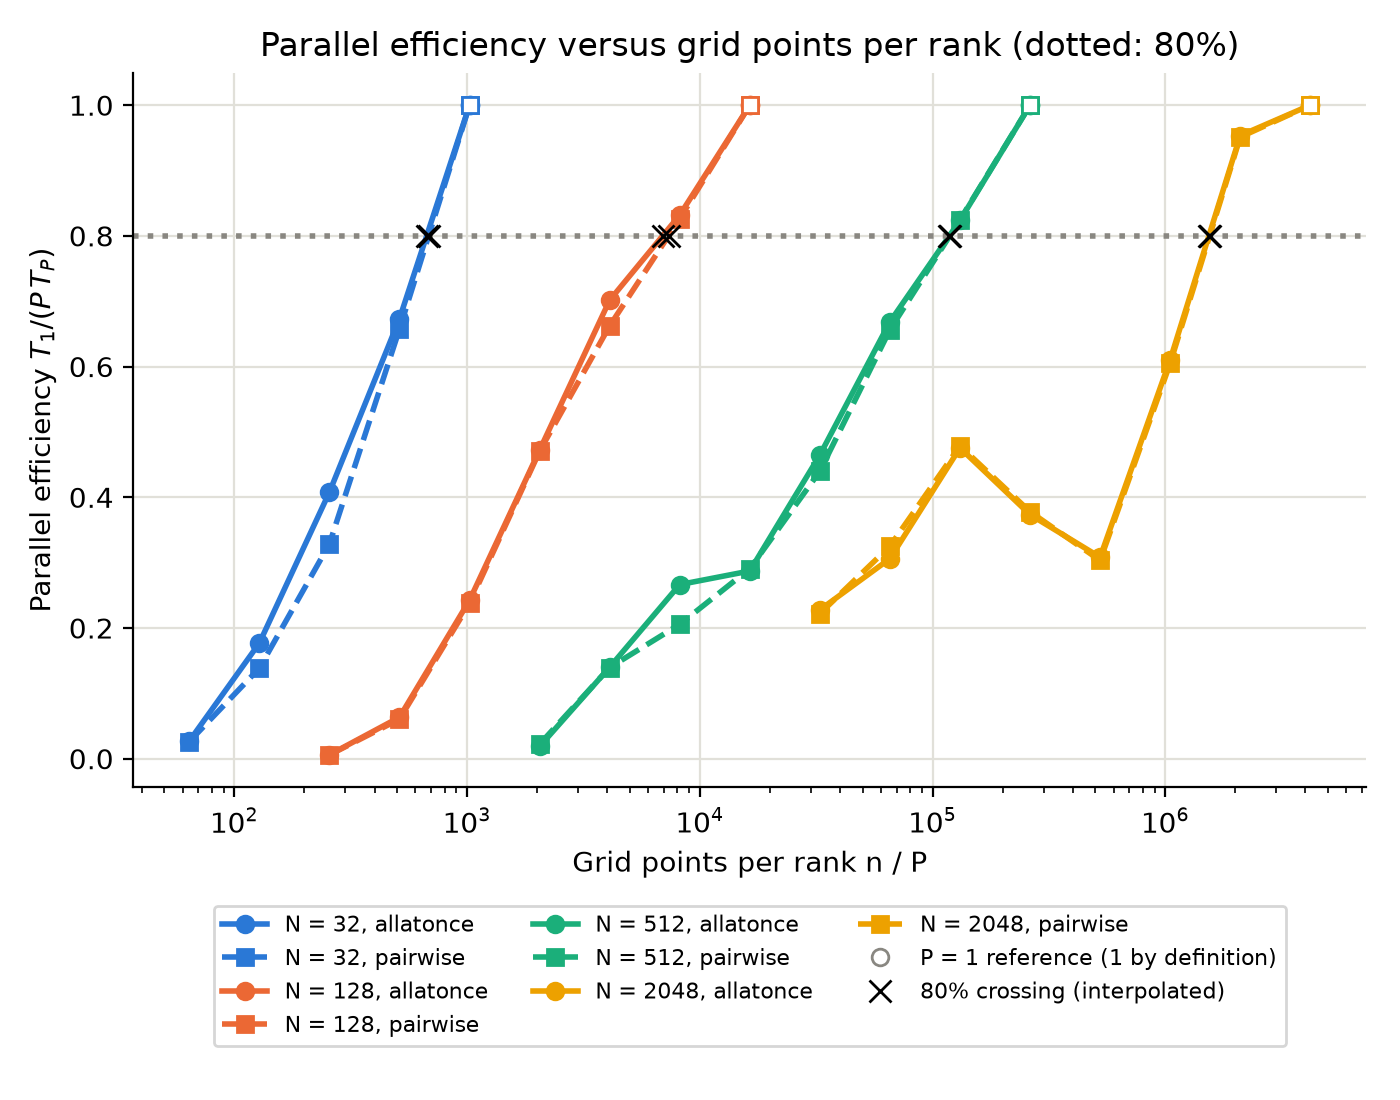
\includegraphics[width=0.6\textwidth]{figures/parallel_efficiency_versus_points_per_rank.png}
  \caption{Parallel efficiency $T_1 / (P \, T_P)$ versus grid points per rank
    $n / P$ for each grid size $N$ and both transpose strategies. The dotted
    line marks 80\% efficiency. Hollow markers are the $P = 1$ reference
    runs, whose efficiency is 1 by definition; crosses mark where each curve
    passes through 80\%.}
  \label{fig:parallel-efficiency-versus-points-per-rank}
\end{figure}

\begin{table}[htbp]
  \centering
  \begin{tabular}{rlcrrr}
    \hline
    $N$  & transpose & bracketing $P$ & $P_{0.8}$ & $n_{0.8} = n / P_{0.8}$ & GFLOPS \\
    \hline
    32   & allatonce & 1 and 2        & 1.53      & 670                     & 5.46   \\
    32   & pairwise  & 1 and 2        & 1.5       & 683                     & 5.35   \\
    128  & allatonce & 2 and 4        & 2.37      & 6.92E+03                & 9.27   \\
    128  & pairwise  & 2 and 4        & 2.23      & 7.33E+03                & 8.71   \\
    512  & allatonce & 2 and 4        & 2.22      & 1.18E+05                & 9.06   \\
    512  & pairwise  & 2 and 4        & 2.21      & 1.18E+05                & 9.06   \\
    2048 & allatonce & 2 and 4        & 2.73      & 1.54E+06                & 8.3    \\
    2048 & pairwise  & 2 and 4        & 2.71      & 1.55E+06                & 8.24   \\
    \hline
  \end{tabular}
  \caption{Rank count $P_{0.8}$, grid points per rank $n_{0.8}$ and aggregate
    GFLOPS at 80\% parallel efficiency. Each curve is interpolated linearly
    in $\log_2 P$ between the two measured rank counts that bracket 80\%, and
    the GFLOPS value is $0.8 \, P_{0.8}$ times the single-rank GFLOPS.}
  \label{tab:efficiency-80}
\end{table}

\begin{table}
  \begin{tabular}{llllll}\end{tabular}
\end{table}


\FloatBarrier

\end{document}
